\chapter{Anforderungsanalyse}
\label{annforderungnsanalyse}
Nachdem die Ziele der Arbeit definiert und bezüglich der einzusetzenden Technik für die Umsetzung die Wahl auf Wearable-Computer (Smartglass) fiel, kann nun die Softwareentwicklung beginnen. Dabei gilt laut Kleucker\footnote{\citep{anforderungsanalyse}} die Anforderungsanalyse als systematischer Einstieg. Deshalb werden in diesem Abschnitt die Anforderungen an das gesamte Softwareprojekt gestellt. Dazu werden zunächst die funktionalen Anforderungen, welche anhand der Arbeitsprozesse aufgeteilt werden, und anschließend die nicht funktionalen Anforderungen erarbeitet und erläutert.\\
In diesem Kapitel werden die Anforderungen hergeleitet und erläutert, allerdings nicht bis ins kleinste Detail analysiert und auch nicht alle Anforderungen vorgestellt. Eine vollständige Liste aller Anforderungen ist dem Anhang zu entnehmen.

\section{Ware einräumen}
Zu Beginn stellt sich die grundsätzliche Frage, wie die Smartglass dem Mitarbeiter überhaupt konkret helfen kann, Ware in das richtige Regal einzuräumen. Die Idee der Nutzung einer Smartglass ist es, dass der Mitarbeiter jederzeit während der Arbeit auf das Display der Datenbrille schauen kann. So kann dem Mitarbeiter angezeigt werden, wo ein entsprechendes Produkt eingelagert werden soll. Dazu erfasst der Mitarbeiter das jeweilige Produkt digital, anschließend zeigt die Smartglass den Lagerort auf dem Display \bzw führt ihn sogar dorthin. Voraussetzung ist eine gegebene Möglichkeit, das Produkt zu erfassen. Darüber hinaus muss die Smartglass eine Zuordnung (Mapping) zwischen dem Barcode und dem Produkt herstellen können.

\begin{itemize}
	\item Anforderung B10: Es gibt eine Möglichkeit, einen Produktcode digital zu erfassen. \label{anforderung_b10}
	\item Anforderung B20: Es gibt eine Möglichkeit, mithilfe des eingescannten Codes ein Produkt zu identifizieren. \label{anforderung_b20}
\end{itemize}

Damit auf dem Display nun der entsprechende Regalplatz angezeigt werden kann, muss die Smartglass in Erfahrung bringen können, wo dieses Produkt einzuräumen ist. Basis für die Visualisierung der Produktposition sind hinterlegte Informationen zu einem Regal und den zugeordneten Produkten. Diese Daten müssen erstellt und verwaltet werden können. Zusätzlich müssen die Daten von der Datenbrille abgerufen werden können, sodass diese damit arbeiten kann. Daraus ergeben sich folgende Anforderungen:

\begin{itemize}
	\item Anforderung A10: Es gibt eine Möglichkeit, Produkte zu administrieren.\label{anforderung_a10}
	\item Anforderung A20: Es gibt eine Möglichkeit, einzelne und mehrere Regale zu administrieren. \label{anforderung_a20}
	\item Anforderung A30: Es gibt eine Möglichkeit, innerhalb der Regale verschiedene Regalplätze zu definieren und diesen einzelne Produkte zuzuordnen. \label{anforderung_a30}
\end{itemize}

Nach einer Produktidentifikation kann nun ein Mapping zu den hinterlegten Produktinformationen vorgenommen werden, um anschließend dem Mitarbeiter \bzw Nutzer der Datenbrille eine Visualisierung anzuzeigen, welche den Mitarbeiter zum entsprechenden Regalplatz eines Produktes führt. Das führt zu folgenden Anforderungen:

\begin{itemize}
	\item Anforderung B40: Es gibt eine Möglichkeit, eine Zuordnung zwischen einem Produkt und dem zugehörigen Regalplatz durchzuführen. \label{anforderung_b40}
	\item Anforderung B40.1: Es gibt eine Möglichkeit, aus der Zuordnung zwischen einem Produkt und seinem Regalplatz eine visuelle Darstellung zu erzeugen und diese dem Nutzer anzuzeigen.\label{anforderung_b40_1}
\end{itemize}

Eine weitere wichtige Hilfe für den Mitarbeiter ist die Benachrichtigung, \textit{wann} ein Produkt eingeräumt werden muss. In der Bedarfsanalyse wurde bereits herausgestellt, dass Mitarbeiter selbst erkennen müssen, dass ein Regalplatz zu wenig Produkte auf Lager hat und aufgefüllt werden muss. Dem Benutzer sollte angezeigt werden, dass ein Produkt eingeräumt werden sollte.\\ 
Dazu ist es erforderlich, dass die Smartglass den Füllstand der Ware auf der Verkaufsfläche und im Lager kennt und der Lagerbestand laufend aktualisiert wird. Es muss also gespeichert werden, wie viel Ware überhaupt vorhanden ist. Zusätzlich ist eine getrennte Erfassung der Lagerbestände im Verkaufsraum und im Lager notwendig, und bei entsprechendem Umräumen (\zB vom Lager in die Regale) auch eine Korrektur der Bestandsinformationen. Die daraus resultierenden Anforderungen sind: 
\begin{itemize}
	\item Anforderung S10: Es gibt eine Möglichkeit, die Lagerbestandsinformationen (von Verkaufsfläche und Lagerraum separat) zu speichern und zu aktualisieren. \label{anforderung_s10}
	\item Anforderung S10.1: Es gibt eine Möglichkeit, dass die Smartglass diese Informationen (automatisch) abrufen kann. \label{anforderung_s10_1}
\end{itemize}

\section{Warenannahme}
Auch die Warenannahme kann mit Unterstützung der Smartglass für den Mitarbeiter vereinfacht werden. Als erster Schritt soll die fehleranfällige analoge Setzliste ersetzt werden. Grundsätzlich muss der Mitarbeiter weiterhin die eingetroffene Ware kontrollieren und zählen, die Erfassung der Ware im System soll nun jedoch von der Smartglass durchgeführt werden, damit hierbei Fehler vermieden werden. Dabei sollte dem Mitarbeiter weiterhin die Bestellung angezeigt werden, damit er ungefähr abschätzen kann, wie viel Ware hätte kommen müssen. Hierzu muss \zB ein Lieferschein erfasst werden, um eine Lieferung eindeutig zu erkennen.\\
Zusammengefasst ergeben sich die Anforderungen der Warenannahme: 

\begin{itemize}
	\item Anforderung B50: Es gibt eine Möglichkeit, mit der Brille die eingetroffene Lieferung zu erfassen und damit die enthaltenen Waren dem aktuellen Lagerbestand hinzuzufügen. \label{anforderung_b50}
	\item Anforderung B60: Es gibt eine Möglichkeit, bei der Warenabnahme die aktuelle Bestellung anzuzeigen. \label{anforderung_b60}
	\item Anforderung B70: Es gibt eine Möglichkeit, einen Lieferschein einzuscannen. \label{anforderung_b70}
\end{itemize}

\section{Kundenzufriedenheit}
Neben den beiden großen Prozessen der Warenannahme und -einräumung ist als Ziel definiert, die Kundenzufriedenheit zu erhöhen. Im Kapitel \ref{sec:bedarf_kundenservice} (\nameref{sec:bedarf_kundenservice}) wurde auf das Problem hingewiesen, dass Kunden Produktinformationen von Personal erfragen wollen und Mitarbeiter sich nicht genügend auskennen. Um das Ziel zu erreichen, ergibt sich folgende Anforderung: 
\begin{itemize}
	\item Anforderung B45: Es gibt die Möglichkeit, den Lagerbestand eines Artikels abzufragen und anzuzeigen. \label{anforderung_b45}
\end{itemize}


\section{Nicht funktionale Anforderungen}

\begin{figure}[H]
	\centering
	{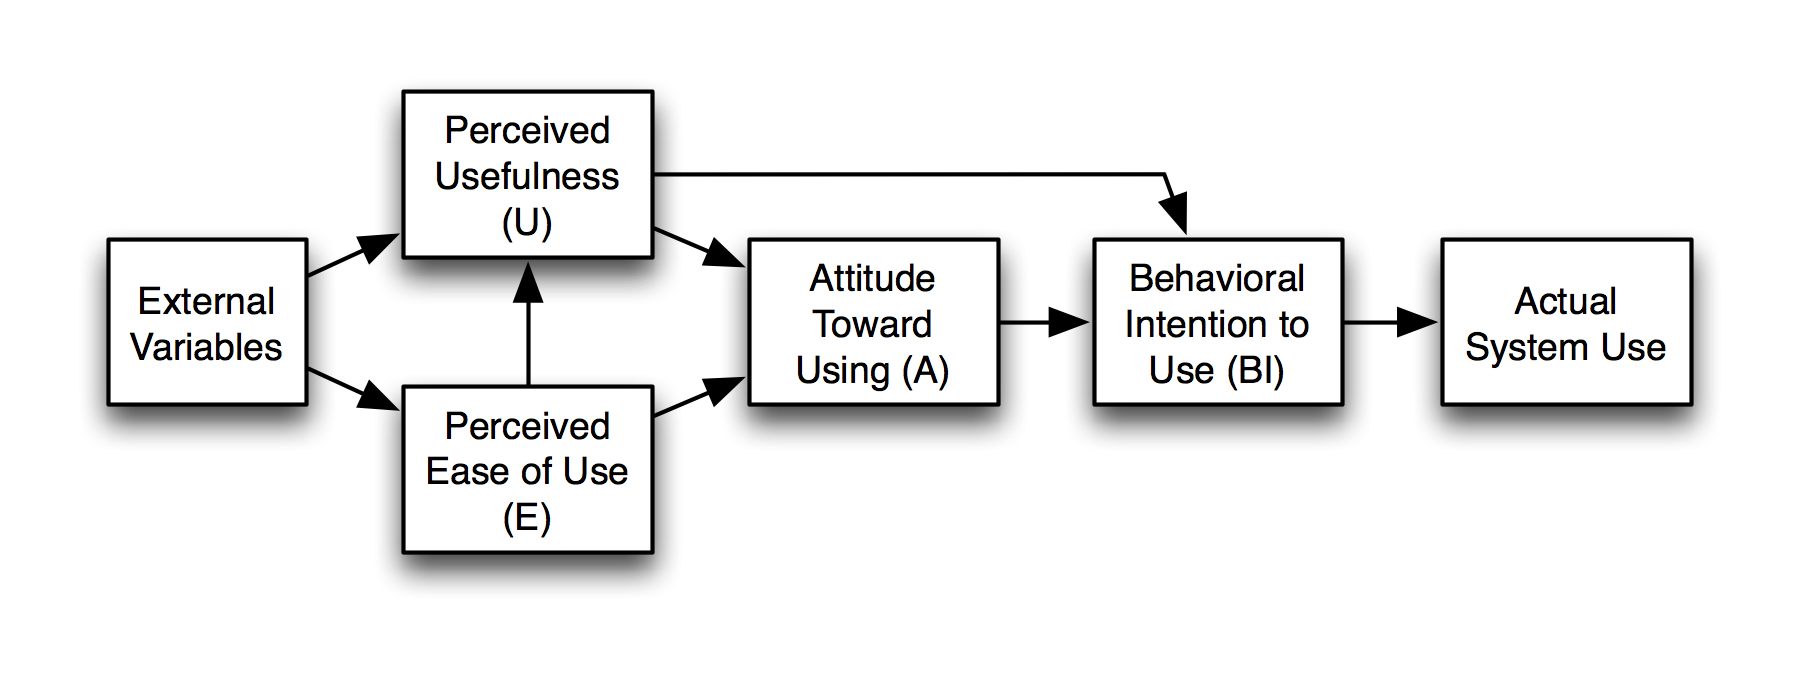
\includegraphics[width=\textwidth]{Bilder/Abbildungen/Technology_Acceptance_Model.png}}
	\caption{Technology Acceptance Model mit externen Einflussfaktoren} 
	\label{fig:tam}
\end{figure}

Neben der eigentlichen Funktionalität spielen die nicht-funktionalen Anforderungen ebenfalls eine große Rolle. Nach dem Technology Acceptance Model (TAM, Version 1)\footnote{Grafik aus: http://commons.wikimedia.org/wiki/File:Technology\_Acceptance\_Model.png} beeinflussen hauptsächlich die \emph{Perceived Usefullness} (empfundener Nutzen) sowie der \emph{Perceived Ease Of Use} (empfundene Einfachheit der Benutzung) als externe Faktoren die Benutzerakzeptanz gegenüber einem System.\footnote{\citep{tam}} Gerade letzterer Punkt wird durch nicht-funktionale Anforderungen abgedeckt. Einer der wichtigsten Punkte ist, dass der Mitarbeiter durch die Smartglass bei seiner Arbeit nicht behindert wird, sonst würde er die Technik nicht akzeptieren und nicht damit arbeiten wollen.\\

Deshalb ist es enorm wichtig, die Performance sehr hoch zu halten. Das bedeutet, dass das System geringe Antwortzeiten anstreben muss, sodass der Nutzer nicht den Eindruck hat, lange auf eine Antwort warten zu müssen. 
Dem Nutzer soll die Bedienung so einfach wie möglich gemacht werden. Damit ist  eine detaillierte und selbsterklärende Menüführung und Anwendungsbeschreibung gemeint, aber gleichzeitig auch der Umgang mit der Smartglass \bzw die Eingaben auf der Brille. \\
Ebenso muss das System robst sein. Das bedeutet, dass das System niemals abstürzen und den Nutzer ohne eine entsprechend aussagekräftige Antwort zurücklassen sollte, da von Mitarbeitern in einer Filiale nicht erwartet werden darf, dass sie sich gut mit solchen Geräten auskennen. Zusätzlich zur Ausfallsicherheit ist die Fehlertoleranz ein entscheidender Faktor. Bei Fehleingaben sollte das System entsprechend reagieren, sodass der Mitarbeiter seinen Fehler erkennt und weiß, was er tun muss, um ihn zu korrigieren und sein Ziel zu erreichen. \\
Eine weitere nicht-funktionale Anforderung ist Energiesparsamkeit. Diese Anforderung entsteht aus dem praktischen Nutzen der Smartglass: Sie muss lange funktionsfähig sein und nicht zu oft aufgeladen werden müssen, weil der Akku leer ist, damit sie sinnvoll eingesetzt werden kann.\\

Die zusammengefassten, nicht-funktionalen Anforderungen lauten:
\begin{itemize}
	\item Anforderung BN1: Die Performance der Smartglass und des Systems ist hoch und erträgliche Antwortzeiten ermöglichen, die den Arbeitsprozess nicht behindern.
	\item Anforderung BN1.10: Das Scannen eines Produktes sollte im Durchschnitt nicht länger als eine Sekunde dauern.
	\item Anforderung BN1.20: Der Abruf der Produktposition inklusive Anzeige des Regalplatzes sollte höchstens 3 Sekunden dauern, im Durchschnitt nur 1,5 Sekunden.
	\item Anforderung BN20: Die Smartglass \bzw deren Software sollte ein hohes Maß an Robustheit aufweisen.
	\item Anforderung BN20.10: Abstürze sollten nicht vorkommen. 
	\begin{itemize}
		\item Anforderung BN20.10.1: Falls doch Abstürze vorkommen sollten, sollte eine beschreibende und zielführende Meldung erscheinen.
	\end{itemize}
	\item Anforderung BN30: Die Software sollte durch Einsparung von Ressourcen möglichst wenig Energie verbrauchen.
\end{itemize}

Die folgende Tabelle enthält alle angesprochenen Anforderungen in einer Übersicht. 
\begin{figure}[H]
	\centering
	{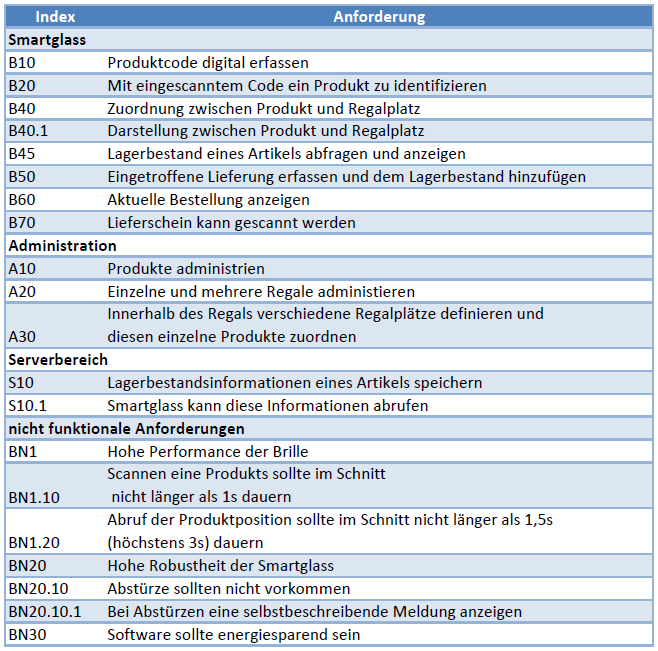
\includegraphics[scale=0.9]{Bilder/Abbildungen/anforderungen_zusammenfassung.png}}
	\caption{Übersicht der wichtigsten Anforderungen}
	\label{fig:anforderungen_uebers}
\end{figure}